\section{Experiments}
\label{sec:experiments}

\subsection{Completed ATE benchmarks}

The completed experiments evaluate ATE estimation only. All nested benchmarks use 20 Monte Carlo repetitions per cell, an RCT-only AIPW baseline, a $\lambda$-only outcome-model fusion estimator, an $\omega$-only PPI correction estimator, and the joint estimator. The code retains two stale internal names: \texttt{haipw\_only} denotes the $\lambda$-only estimator and \texttt{ppi\_power\_tuned\_only} denotes the $\omega$-only estimator. The first label does not identify the method with the separate HAIPW literature.

\begin{figure}[htbp]
\centering
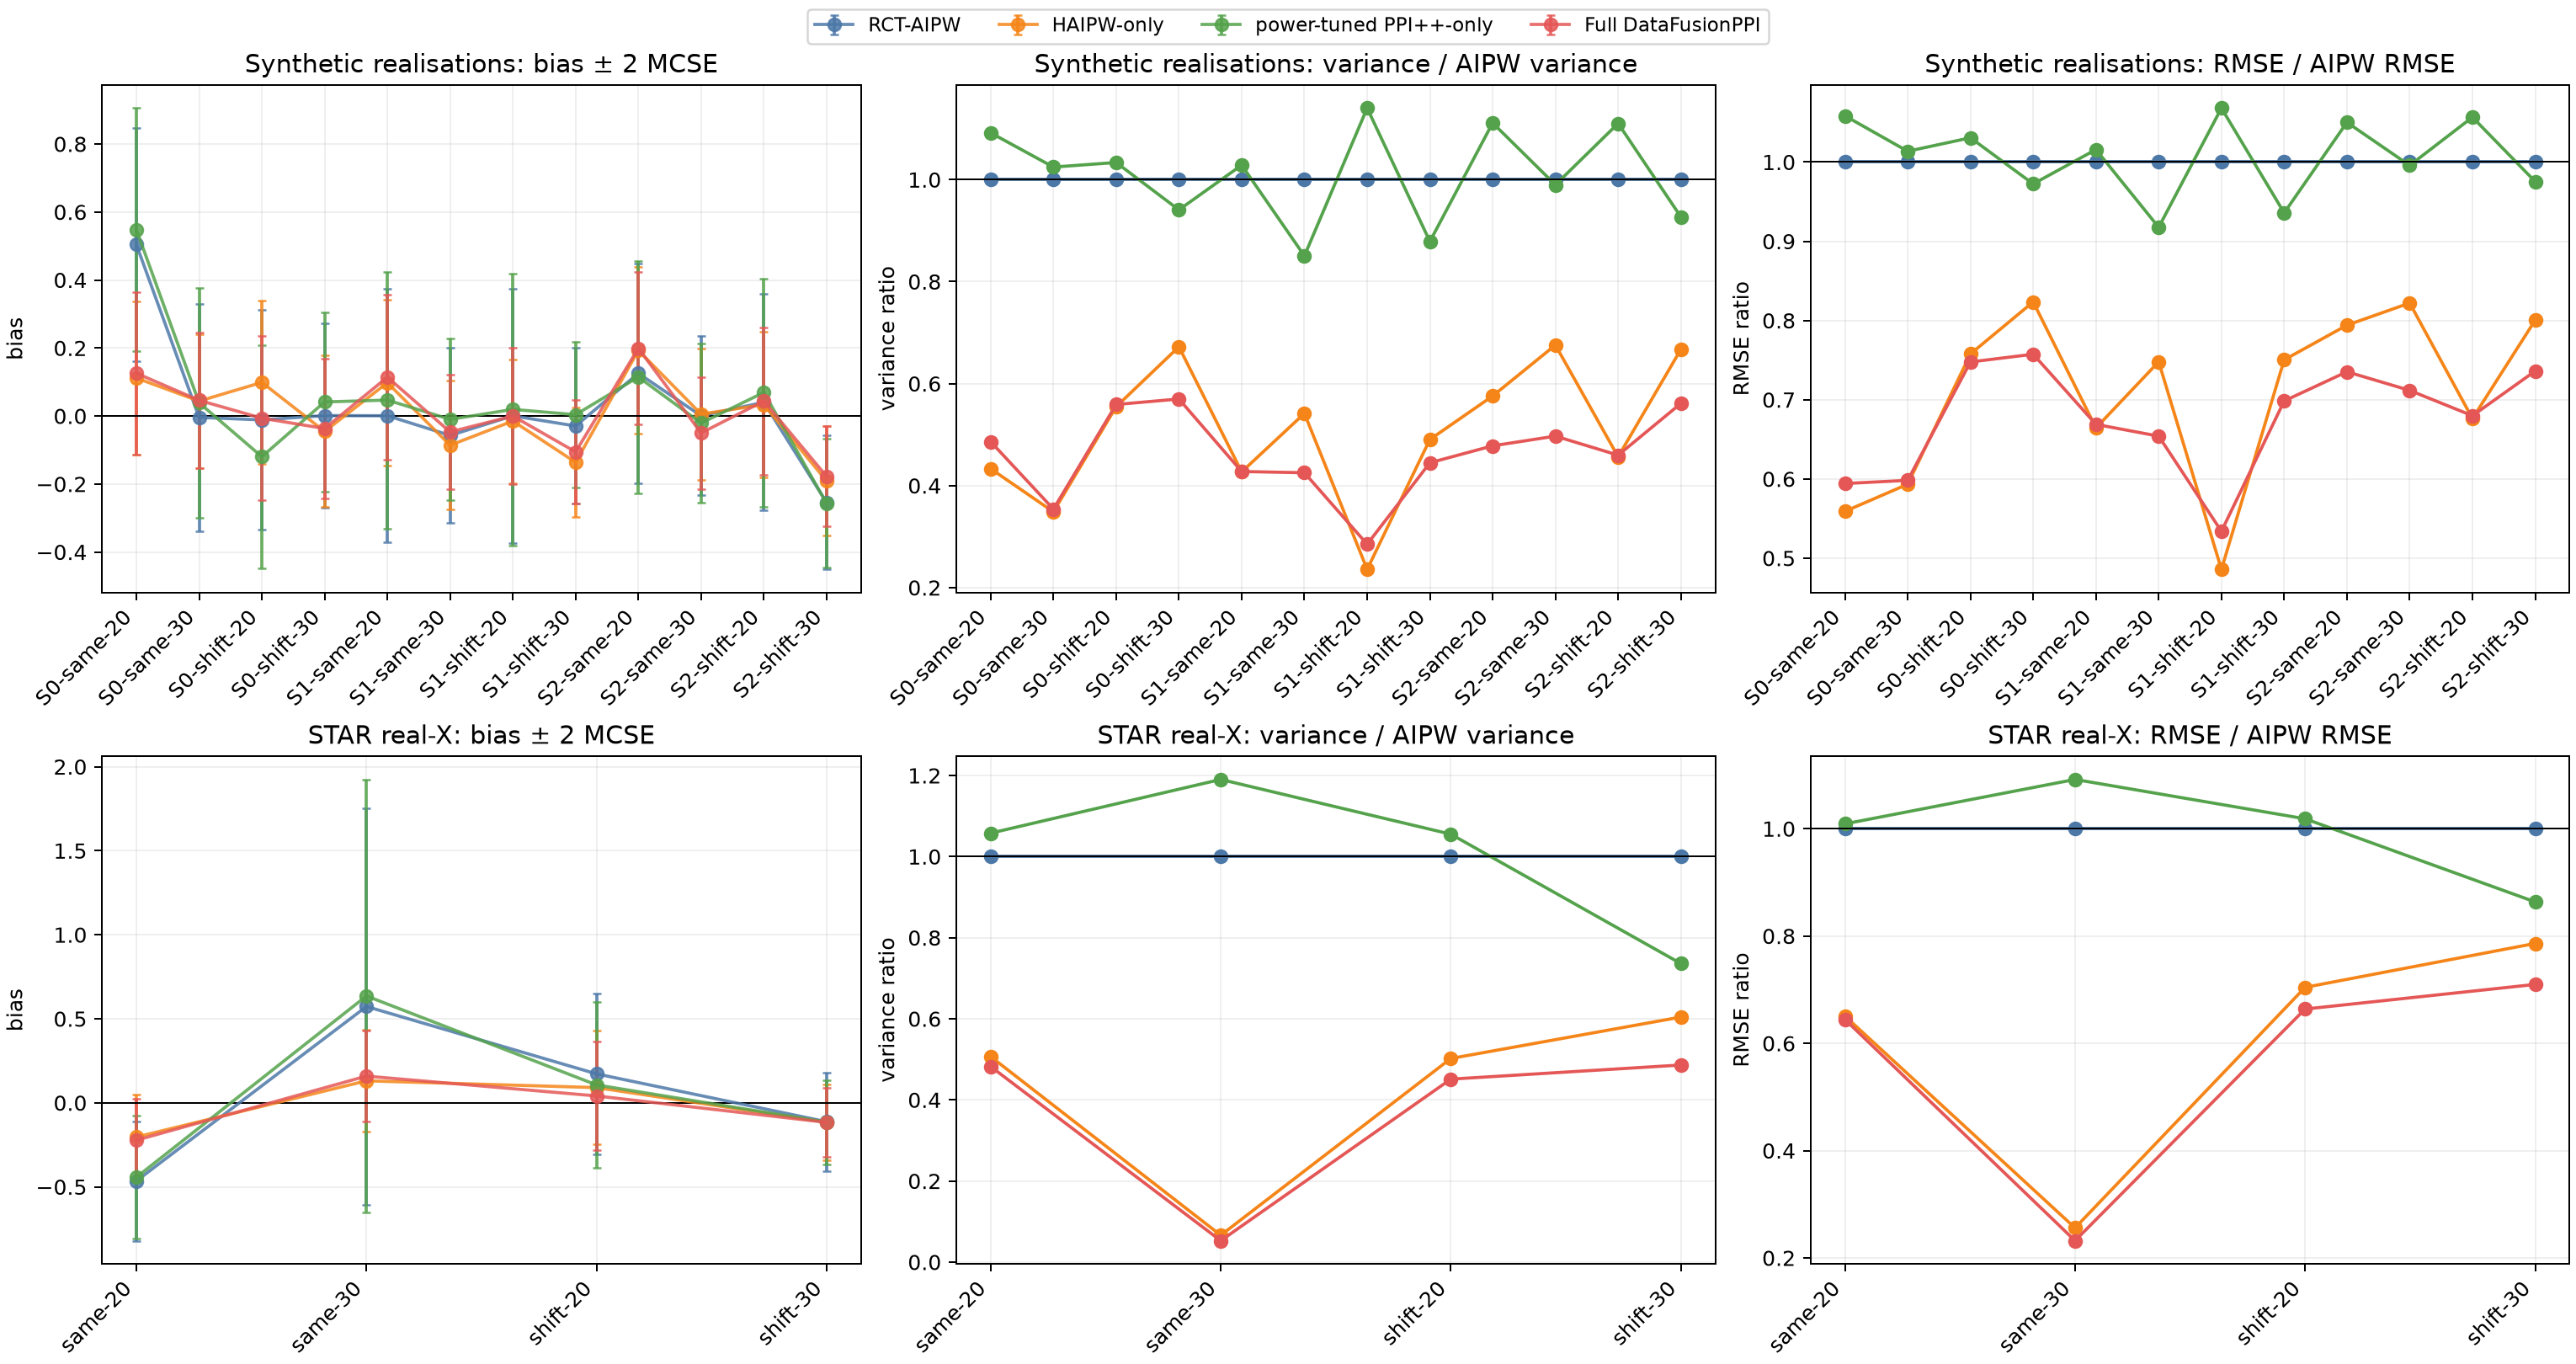
\includegraphics[width=0.98\textwidth]{../materials/total_budget_nested_benchmark.png}
\caption{Fixed-OBS-budget ATE benchmark. The composite artifact reports multiple method and regime panels side by side for $n_R\in\{20,30\}$ and $N_O=5000$.}
\label{fig:fixed-budget}
\end{figure}

\begin{figure}[htbp]
\centering
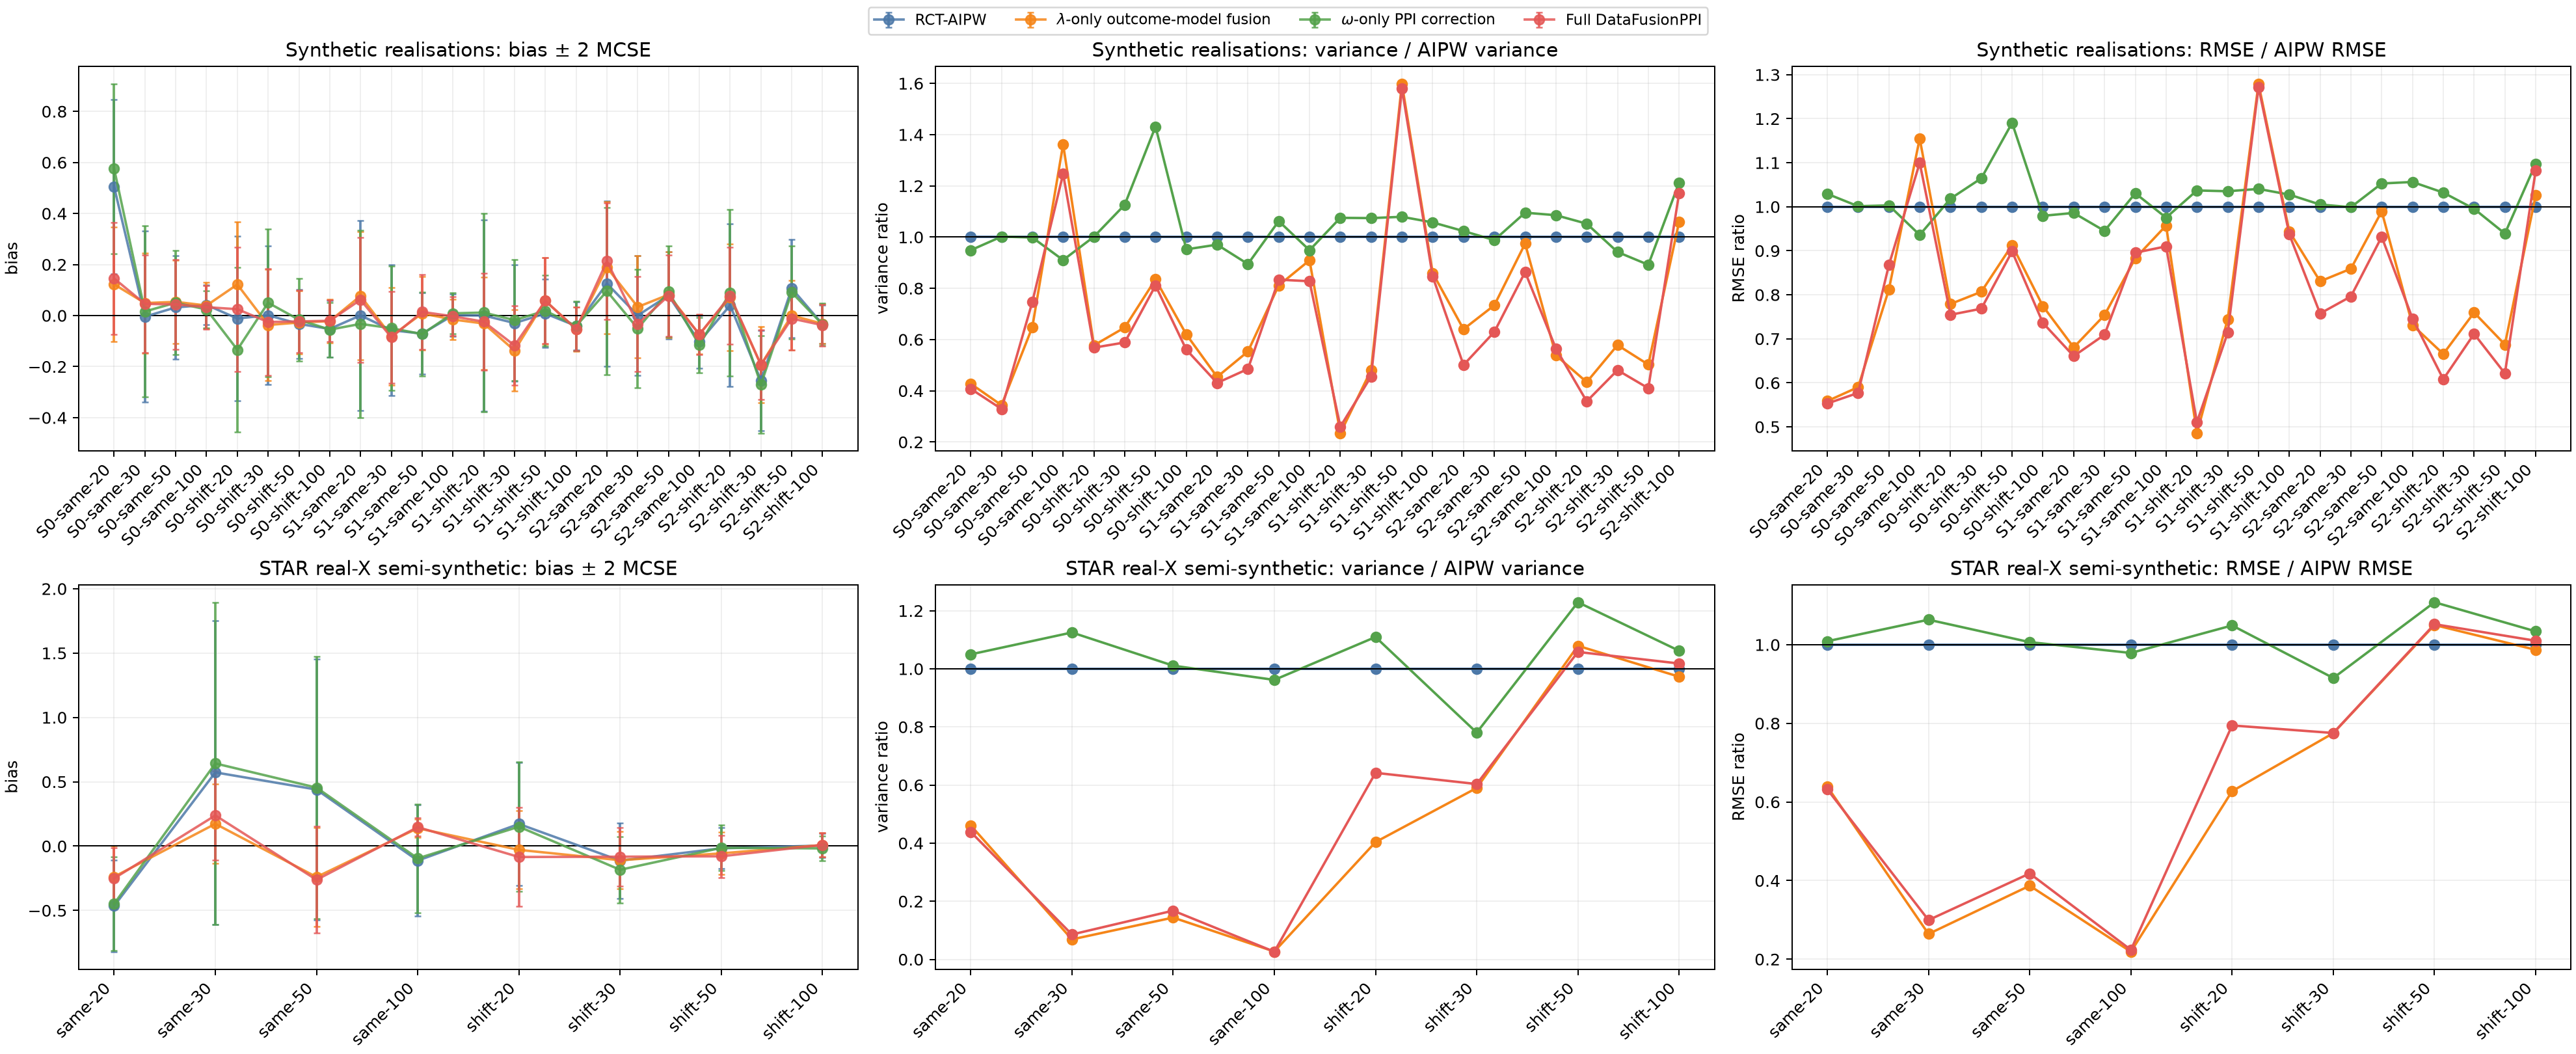
\includegraphics[width=0.98\textwidth]{../materials/proportional_budget_nested_benchmark.png}
\caption{Proportional-budget ATE benchmark. The composite artifact reports multiple method and regime panels side by side for $n_R\in\{20,30,50,100\}$ and $N_O=100n_R$.}
\label{fig:proportional-budget}
\end{figure}

The fixed-OBS-budget benchmark contains 16 design cells: three arbitrary nonlinear SCMs and one STAR real-$X$ construction, each under a common covariate marginal and covariate shift and $n_R\in\{20,30\}$, with $N_O=5000$. The joint estimator has the smallest RMSE in 11 cells, and the $\lambda$-only estimator is best in the remaining five. The joint estimator has lower RMSE than AIPW in all 16 cells, with mean RMSE ratio $0.648$ and mean empirical-variance ratio $0.439$ relative to AIPW. The $\lambda$-only estimator also beats AIPW in all 16 cells, with mean RMSE ratio $0.679$. The $\omega$-only estimator is not best in any cell and has mean RMSE ratio $1.005$.

The proportional-budget benchmark contains 32 cells with $n_R\in\{20,30,50,100\}$ and $N_O=100n_R$. The joint estimator has the smallest RMSE in 18 cells, the $\lambda$-only estimator in 10, the $\omega$-only estimator in one, and AIPW in three. The joint estimator has lower RMSE than AIPW in 27 of 32 cells, with mean RMSE ratio $0.760$ and mean empirical-variance ratio $0.625$. The $\lambda$-only estimator beats AIPW in 28 cells and has mean RMSE ratio $0.769$. The $\omega$-only estimator beats AIPW in 10 cells and has mean RMSE ratio $1.020$. These counts show that joint tuning is often useful but is not uniformly best after coefficient estimation.

The STAR benchmark uses only real kindergarten covariates from Project STAR. Treatment assignments, latent confounding, potential outcomes, and effect heterogeneity are generated synthetically. It is therefore a real-$X$, semi-synthetic benchmark rather than an analysis of STAR's original intervention or outcomes. The planned WHI CT+OS analysis has not been run because participant-level access, a semantic crosswalk, and a survival or censoring extension are still required.

\subsection{Planned CATE evaluation and interpretation}

CATE experiments are planned. The primary design will compare the proved AIPW-pseudo-outcome F-Learner with the prospective R-loss extension using additive cubic B-splines, frozen neural bases, and linear sieves under a common covariate marginal and covariate shift. Each study will compare trial-only, $\lambda$-only, $\omega$-only, and joint tuning using held-out RCT-population CATE risk. Classifier-only, balancing-only, hybrid, and oracle transport weights will be separated. No CATE result is claimed from Figures~\ref{fig:fixed-budget} and \ref{fig:proportional-budget}.

The empirical conclusion is deliberately limited. The two-channel population oracle weakly improves the ATE variance objective when the trial-only coefficient is feasible, but estimated coefficients do not inherit a universal no-harm property. The present 20-repetition studies suggest that the $\lambda$ channel is the more stable source of gain and that joint tuning can add value in some designs. More Monte Carlo repetitions, completed CATE experiments, additional real-$X$ supports, and an authorized real-outcome analysis are required before making a stronger empirical claim.

\subsection{Scope, failure modes, and conclusion}
\label{sec:active-conclusion}

The framework uses observational information through prediction rather than by declaring the observational treatment contrast causal. Trial randomization validates the pseudo-outcome for every fixed outcome regression. A common covariate marginal or an exact density ratio centers the ATE control variate and the prediction-powered CATE loss, which creates separate $\lambda$- and $\omega$-channels while retaining RCT-population targets.

The first boundary is covariate transport. Without weighting under $P_R^X\neq P_O^X$, the ATE correction has drift $\omega\{P_O\widehat{g}-P_R\widehat{g}\}$, and the unweighted CATE loss targets the wrong covariate average. Exact $r=dP_R^X/dP_O^X$ removes both discrepancies. An estimated ratio instead contributes the explicit ATE drift $\omega P_O\{(\widehat r-r)\widehat{g}\}$ and the CATE validation drift in item 3 of Theorem~\ref{thm:cate-finite-validation}. Evaluation-only variance is first-order adequate only under the stated negligible-drift conditions; otherwise ratio-training influence and covariance terms are required.

The second boundary is trial propensity overlap. Proposition~\ref{prop:pseudo-validity-active} uses the known, strictly positive randomized-trial propensity. Extreme inverse-propensity factors can make the required moments unstable even when the conditional-mean identity remains algebraically valid, and an incorrect propensity removes the exact arbitrary-$q$ guarantee.

The third boundary is weak observational prediction. The unrestricted $\omega$-gain depends on how strongly $\widehat{g}(X)$ predicts $\tau(X)$, with attenuation from the finite $n/N$ ratio. The $\lambda$-channel gives little gain when $\Delta=Z_1-Z_0$ is uninformative or nearly degenerate. Population oracles diagnose these limits but do not make their empirical coefficient estimates stable.

The fourth boundary is adaptive reuse. Fitting nuisances, tuning candidates, and evaluating the selected candidate on the same outcomes invalidates the conditioning product law. Present inference therefore uses independent nuisance-fitting, coefficient-tuning, and final-evaluation samples, supplied separately or constructed by splitting. The theory does not cover cross-fitted reuse; that extension requires a separate stability or influence-function analysis.

The fifth boundary is learner restriction and curvature. Target preservation does not make a finite-sample restricted or highly penalized projection accurate. The square-completed representation is a nonnegative mixture only for $0\leq\omega<1$, and positive semidefiniteness at $\omega=1$ must be read from the original quadratic. Coefficients outside $[0,1]$, nonlinear parameterizations, and penalty rescaling require direct analysis of the original objective.

The sixth boundary is tail behavior. ATE variance identities require square-integrable scores; the Wald theorem additionally requires conditional Lindeberg control, a sufficient $(2+\delta)$-moment condition, and a nondegenerate variance limit. Fixed-loss variance tuning imposes fourth-moment-type requirements. Heavy tails can therefore destabilize oracle formulas even when their algebraic denominators are nonzero.

Within these boundaries, the randomized trial fixes the causal target, the OBS outcome model can reduce within-$X$ pseudo-outcome noise through $\lambda$, and the OBS covariate sample can reduce predictable between-$X$ variation through $\omega$. The exact results are conditional identities and population-oracle comparisons. Empirical work must retain the identical trial-only fallback, report selection and denominator instability, and avoid interpreting them as a universal finite-sample no-harm guarantee.
